\documentclass[a4paper,12pt]{article}
\usepackage [left=25.4mm,top=25.4mm]{geometry}
\usepackage{amsmath}
\usepackage{amssymb}
\usepackage{graphicx}
%\usepackage{apacite}
\usepackage{url}
\usepackage{subfig}
\usepackage{csvsimple}
\usepackage{float}
\usepackage{lineno}
\usepackage[affil-it]{authblk}
\usepackage{setspace}
\usepackage{makecell} 
\usepackage{tikz}
\usepackage{csvsimple}
\usepackage{newfloat}
\usepackage{xcolor}
\usepackage{tabularx,booktabs}
\usepackage{multirow}
\usepackage{multicol}
\usepackage{array}
\usepackage{tocbasic}
\usepackage{sectsty}

\sectionfont{\fontsize{12}{15}\selectfont}
\chapterfont{\fontsize{14}{15}\selectfont}
\subsectionfont{\fontsize{10}{15}\selectfont}

\newcommand\hcancel[2][black]{\setbox0=\hbox{$#2$}%
	\rlap{\raisebox{.45\ht0}{\textcolor{#1}{\rule{\wd0}{1pt}}}}#2} 
\newcommand{\forceindent}{\leavevmode{\parindent=2em\indent}}

\DeclareFloatingEnvironment[name={Supplementary Figure},fileext=lsf,listname={List of Supplementary Figures}]{suppfigure}
\DeclareFloatingEnvironment[name={Supplementary Table},fileext=lsf,listname={List of Supplementary Tables}]{supptable}
\DeclareFloatingEnvironment[name={Supplementary Material},fileext=lsf,listname={List of Supplementary Material}]{suppmat}

\newcolumntype{P}[1]{>{\centering\arraybackslash}p{#1}}
\newcolumntype{M}[1]{>{\centering\arraybackslash}m{#1}}

\DeclareMathOperator*{\argmax}{arg\,max}
\DeclareMathOperator*{\argmin}{arg\,min}

\newcommand{\indep}{\perp \!\!\! \perp}
\renewcommand*\contentsname{TABLE OF CONTENTS}
\renewcommand{\listfigurename}{LIST OF FIGURES}
\renewcommand{\listtablename}{LIST OF TABLES}

\renewcommand{\arraystretch}{1.5}
\begin{document}
	\begin{titlepage}
		\title{HGRN Algorithm}
		\author[1]{Jarred M. Kvamme}
		\author[2]{Boyu Zhang}
		\author[1,3]{Audrey Q. Fu}
		\affil[1]{Department of Bioinformatics and Computational Biology - University of Idaho}
		\affil[2]{Department of Computer Science - University of Idaho}
		\affil[3]{Department of Mathematics and Statistical Science - University of Idaho}
		\maketitle
	\end{titlepage}
	
	
	\newpage
	\tableofcontents{}
	\addcontentsline{toc}{section}{LIST OF TABLES}
	\addcontentsline{toc}{section}{LIST OF FIGURES}
	\listoftables
	\listoffigures
	\newpage
	
	
	
	
	
	\section{Preprocessing}
	\begin{itemize}
		\item[\bf 1.1]{\textbf{Graph Initialization}: Given an attributed network $\mathcal{G}_0(E,V,{\bf X})$ with attribute matrix ${\bf X} =\{x_1, x_2;...;x_N\} \in \mathbb{R}^{N \times p}$ where $\bf x_i$ is the $p$-length attribute vector of node $n_i$, $E = \{ (v_i, v_j)| 1<i, j<N, i\neq j\}$ edges, and $V = \{v_i\}_{i=1}^N$ nodes/vertices, estimate an initial graph of $\bf X$ represented by the adjacency matrix ${\bf A} \in \mathbb{R}^{N\times N}$ 
		\begin{itemize}
			\item[1.1.1]{\textbf{Correlations method:} Compute the correlation matrix ${\bf R}\in[0,1]^{N\times N}$ from $\bf X$. Convert the correlation matrix $\bf R$ into an adjacency matrix ${\bf A}_0$ such that 
				\[ \hat{a}_{i,j} = \begin{cases}
					1 & \text{if} \ \  r_{i,j} > \rho \\
					0 & \text{else}
				\end{cases} \] 
			where $\rho$ represents a minimum correlation threshold to consider an edge $(v_i, v_j)$ between nodes $i$ and $j$.}
			
			\item[1.1.2]{\textbf{K-neighbors method:} }
			
			\item[1.1.3]{\textbf{Precision method:}}
		\end{itemize} }
	
	\item[1.2]{\textbf{Estimate Hierarchical Structure}:} 
		
	\end{itemize}
	
	\section{Training}
	\begin{itemize}
	\item[\bf 2.1]{\textbf{Initialize HGRN Model} \\
		Input: The model takes as input the attributed graph represented by the adjacency matrix and node attribute matrix $\{{\bf A}, {\bf X}\}$, respectively. \\
		\\
		Parameters: \textbf{Number of hierarchical layers} ($\ell$), \textbf{communities per layer} ($K =\{k_i\}_{i=1}^\ell$), \textbf{max training epochs} ($t$) \\
		\\
		Output: The output includes the reconstructed node attribute matrix $\hat{\bf X}$ and adjacency matrix $\hat{\bf A}$ as well as the node assignments the hierarchy \textbf{hierarchical graph} ($\mathcal{H} = \{\mathcal{G}_i\}_{i = 0}^\ell$
	}

	\item[\bf 2.2]{\textbf{For $t$ Epochs}:}
		\begin{enumerate}
			\item[2.2.1]{\textbf{Compute forward pass}: \\
			
			 \forceindent \textbf{Encoder Module}: \\
			 \forceindent \textbf{For $m$ encoder layers}: 
			\begin{enumerate}
				\item[]{We adopt the graph attention autoencoder \textbf{GATE} proposed by \cite{salehi2019graph} which consists of graph attention based encoder and decoder models that reconstruct the original graph ${\bf A}$ and the node feature matrix $\bf{X}$}
				\item[]{\textbf{$\bullet$ Attention weights} \\
					The GAT mechanism applies additional trainable parameters ${\bf a}$ to the neighbors of each node to learn their relevance given by the weight $\theta_{i,j}$. The attention weight $\theta_{i,j}$ represents the importance of node $i$ in the representation of $j$ For the GAT model, the relevance of node neighbors (i.e their attention weights) is computed via the following:
					
					\[ \theta_{ij} = \frac{\sigma\left(\exp\left({\bf a}_s^T\phi\left[{\bf W}h_i\right]+{\bf a}_v^T\phi\left[{\bf W}h_j \right]\right)\right)}
					{\sum_{k\in \mathcal{N}(i)}\sigma\left(\exp\left({\bf a}_s^T\phi\left[{\bf W}h_i\right]+{\bf a}_v^T\phi\left[{\bf W}h_k \right]\right)\right)} \]
					The weight parameters ${\bf a}_s^T$ aim to capture additional semantic information in node $i$ while the weight parameter ${\bf a}_v^T$ captures semantic information in node $j$. Furthermore, the Softmax function is used to normalize the attention coefficients so that the coefficients in the neighborhood of node $i$ sum to 1. \\
					\\
					In linear form, the [matrix of] attention coefficients for the $m$ layer of the model ${\bf \Theta}^{(m)}$ are computed as 
					\[{\bf \Theta}^{(m)} = \text{Softmax}\left(\sigma\left({\bf M}_s^{m} + {\bf M}_v^{m}\right)\right) \]
					\[{\bf M}_s^{m} = {\bf A}\odot \left[{\bf a}_s^{(m)^T} \cdot \phi\left({\bf W}_{m}{\bf H}_{m-1}\right)\right]\]
					\[{\bf M}_v^{m} = {\bf A}\odot \left[{\bf a}_v^{(m)^T}\cdot \phi\left( {\bf W}_{m}{\bf H}_{m-1}\right)\right]^T\]
					
					where
					\[ {\bf \Theta}_{ij}^{(m)} = \begin{cases} \theta_{ij}^{(m)} & \text{if there is and edge between node $i$ and node $j$} \\ 0 & \text{else}\end{cases} \]
					
					Note that in the above equations $\sigma$ is the sigmoid logistic function, $\odot$ denotes the element-wise product operation between matrices, and $\phi$ denotes the layer activation function. In the original formulation of GAT by \cite{velivckovic2017graph}, $\phi$ was the identity function, and LeakyReLU was used in place of the sigmoid funciton.}\\
					
				\item[]{\textbf{$\bullet$ Compute encoder hidden layers}
					By considering $H_0 = X$, the $m-1^{th}$ encoder layer generates node
					representations in hidden layer $m-1$ as follows:
					
					\[ {\bf H}_{m-1} = \sigma\left({\bf W}_{m-1}\cdot {\bf H}_{m-2}\right)\cdot {\bf \Theta}^{(m-1)}\] 
					Where ${\bf \Theta}_{m}$ is the matrix of attention coefficients for layer $m-1$\\
					}
				\newpage
				\item[]{\textbf{$\bullet$ Compute embedding dimension} \\
					The embedding or bottleneck dimension follows the same format above as fully connected GAT layer which takes the ($m^{th}$) hidden layer of the encoder as input.
					\[ {\bf Z} = \sigma\left({\bf W}_m\cdot {\bf H}_{m-1}\right)\cdot {\bf \Theta}^{(m)}\]
					
					} 
			\end{enumerate}
			\forceindent \textbf{Decoder Module}: \\
			\forceindent \textbf{For $m$ decoder layers}:
			\begin{enumerate}
				\item[]{\textbf{$\bullet$ Attention weights} \\
					The attention weight of the decoder layers are computed in similar fashion where $\theta_{i,j}$ represents the importance of node $i$ in the representation of $j$:
					
					\[ \hat{\theta}_{ij} = \frac{\sigma\left(\exp\left({\bf a}_s^T\phi\left[{\bf \hat{W}}\hat{h}_i\right]+{\bf a}_v^T\phi\left[{\bf \hat{W}}\hat{h}_j \right]\right)\right)}
					{\sum_{k\in \mathcal{N}(i)}\sigma\left(\exp\left({\bf a}_s^T\phi\left[{\bf \hat{W}}\hat{h}_i\right]+{\bf a}_v^T\phi\left[{\bf \hat{W}}\hat{h}_k \right]\right)\right)} \]
					\\
					Where the matrix of attention coefficients for the $m^{th}$ decoder layer is defined as:
					\[{\bf \hat{\Theta}}^{(m)} = \text{Softmax}\left(\sigma\left({\bf \hat{M}}_s^{m} + {\bf \hat{M}}_v^{m}\right)\right) \]
					\[{\bf \hat{M}}_s^{m} = {\bf A}\odot \left[{\bf \hat{a}}_s^{(m)^T} \cdot \phi\left({\bf \hat{W}}_{m}{\bf \hat{H}}_{m-1}\right)\right]\]
					\[{\bf \hat{M}}_v^{m} = {\bf A}\odot \left[{\bf \hat{a}}_v^{(m)^T}\cdot \phi\left( {\bf \hat{W}}_{m}{\bf \hat{H}}_{m-1}\right)\right]^T\]
					
					where
					\[ {\bf \hat{\Theta}}_{ij}^{(m)} = \begin{cases} \hat{\theta}_{ij}^{(m)} & \text{if there is and edge between node $i$ and node $j$} \\ 0 & \text{else}\end{cases} \]
					}\\
				\item[]{\textbf{$\bullet$ Compute decoder hidden layers.}\\
					The decoder layers also consist of $m$ GAT layers under the GATE model architecture. We use $\hat{\bf H}$ notation to denote the layers of the decoder as reconstructions of the embeddings $\bf Z$. The first decoder layer takes the embedding matrix $\bf Z$ as the feature information for the nodes and outputs the hidden decoder layer $\hat{\bf H}_1$ 
					\[ {\bf \hat{H}}_{1} = \sigma\left({\bf \hat{W}}_{1}\cdot {\bf Z}\right)\cdot {\bf \hat{\Theta}}^{(1)}\]
				}\\
				\item[]{\textbf{$\bullet$ Reconstruct the input from the final decoder}
					following \cite{salehi2019graph} we take the reconstructed node attributes as the final layer of the decoder:
					
					\[\hat{\bf X} = {\bf \hat{H}}_m = \sigma\left({\bf \hat{W}}_{m}\cdot {\bf \hat{H}}_{m-1}\right)\cdot {\bf \hat{\Theta}}^{(m)}\]
				}\\
				
				\item[]{\textbf{$\bullet$ Graph reconstruction} 
					Following \cite{kipf2016semi, salehi2019graph, zhou2023community}, we reconstruct the adjacency matrix of the attributed graph from the embedding dimension using a simple dot-product decoder function activation: 
					\[\hat{\bf A} = \sigma\left(Z\cdot Z^T\right) \]
					As usual, $\sigma$ denotes the sigmoid (logistic) activation function which assumes a normal distribution and transforms the weights of the adjacency matrix into pseudo-probabilities of node linkages: $\hat{\bf A} \in [0,1]^{N\times N}$
				}\\
					
			\end{enumerate}
			\forceindent \textbf{Super-Node Classification Layers}: \\
			\forceindent \textbf{For $\ell+1$ hierarchical layers}:
			\begin{enumerate}
				\item[]{\textbf{$\bullet$ Compute community assignment probabilities} 
					\\
					In this step we construct $\ell$ single layer linear classifiers. Each linear classifier will output the community assignments of nodes (or super-nodes) from the previous layer. The first linear classifier uses the embeddings to classify $N$ nodes to $k_1$ communities given by
					\[{\bf P}_{1} = \text{Softmax}\left({\bf Z}{\bf W}_{1}\right) \]
					\\ 
					\[= \begin{bmatrix}
						p_{1, 1} & \cdots & p_{1, k_\ell} \\
						\vdots  & \ddots & \vdots \\
						p_{k_{\ell - 1}, 1} & \cdots & p_{k_{\ell -1}, k_\ell} 
					\end{bmatrix}\]}\\
				
					Where $\bf P$ is a matrix with nodes in the rows and assignment probabilities in the columns. For example, the $i$ row of ${\bf P}_1$ represent the probabilities for assigning  node $i$ to each of the $k_1$ communities. The Softmax function therefore regularizes the rows of ${\bf P}_1$ such that the sum of the probabilities equals one and each row represents a valid probability distribution for assigning nodes to communities. \\
					
				
				%\item[]{\textbf{$\bullet$ Normalize the community assignment probabilities}
			%		\\
				%	In this step the community assignment probabilities are normalized according to the method of \cite{zhou2023community} 
			%		\[ \hat{p}_{i,k_\ell} = \frac{\sqrt{k_{\ell-1}} \sqrt{p_{i, k_\ell}}}{\sum_i \sum_{k_\ell} \sqrt{p_{i, k_\ell}}}\]
					
			%		\[\hat{\bf P}_\ell = \begin{bmatrix}
			%			\hat{p}_{1, 1} & \cdots & \hat{p}_{1, k_\ell} \\
			%			\vdots  & \ddots & \vdots \\
			%			\hat{p}_{k_{\ell - 1}, 1} & \cdots & \hat{p}_{k_{\ell -1}, k_\ell} 
			%		\end{bmatrix}\]
			%	}
				
				
				\item[]{\textbf{$\bullet$ Compute community assignment labels} \\
					The community assignment matrix is a boolean matrix which represents the community assignment of a node or super node such that the $c_{i,j}^{(\ell)} = 1$ at the $k_\ell^{th}$ position if a node is assigned to community $k_\ell$ and zero otherwise. This matrix can be obtained by taking the argument maximum over the rows of community assignment probabilities ${\bf P}_\ell$ for the $\ell^{th}$ hierarchical layer.  
					\[{\bf C}_{\ell} = g({\bf P}_{\ell}) \ \text{where} \ \  g(\hat{p}_{i,k_\ell}) = 
					\begin{cases} 1 & \ \text{if} \ \ \text{node $i$ assigned to community $k_\ell$} \\ %\in \mathcal{C}^{\ell}_{k_\ell} \\
						0 & \text{else} %\ v_i \not\in \mathcal{C}^{\ell}_{k_\ell}
					\end{cases}\]\\
				
				
					For each hierarchical layer $\ell$ we may compute the community assignment labels. Consider a two-layer hierarchy, the community assignment labels $\mathbb{S}_1$ from assigning $N$ nodes in the bottom layer to $k_1 < N$ nodes in the super layer is given as 
					\[\mathbb{S}_1 = \argmax_{k_1} {\bf C}_1 \]
					
					more generally, the labels from assigning nodes in layer $\ell - 1$ to layer $\ell$ is given as:
					
					\[ \mathbb{S}_\ell = \argmax_{k_\ell} {\bf C}_{\ell}\]
				}
				
				\item[]{\textbf{$\bullet$ Compute input to the next classifier:}  \\
					Each linear classifier aims to classify the nodes in the previous layer to a subset of nodes which represent the communities of the current layer. For example, the first classifier classifies the $N$ original nodes to $k_1$ communities and takes as input the embeddings matrix from the auto-encoder. The second classifier which classifies $k_1$ communities to $k_2$ communities takes as input the centroids of the $k_1$ communities in the previous layer which is computed by projecting the embeddings onto the community probabilities matrix ${\bf P}_1$. These centroids are then activated to ensure regularity denoted by the activation function $\phi(\cdot)$ which may be the identity function:
					\[ {\bf \tilde {X}}^{(1)}= \phi\left({\bf Z}^T {\bf P}_{1}\right)^T\] 
					\\
					Thus ${\tilde \bf X}^{(1)} \in \mathbb{R}^{k_1 \times q}$ is matrix corresponding the centroids of the $k_1$ predicted communities in $q$ embedded features. In general, for layers $\ell > 1$ in the hierarchy, the input is calculated from the linear combination of the centroids of the previous layer $\ell - 1$ and with the community assignment matrix of the current layer $\ell$ and activated by function $g_\ell(\cdot)$: 
					\[ {\bf \tilde X}^{(\ell)} = \phi_\ell\left({\bf \tilde{X}}^{(\ell-1)^T} {\bf P}_{\ell}\right)^T\] 
					\\
					
					Since our main objective is to learn the hierarchical representation of the original graph, we also compute the adjacency matrices corresponding to each hierarchical layer. We want the adjacency matrix for a given hierarchical layer to summarize the connections between and within the communities of that layer. For example, assigning the $N$ original nodes to $k_1$ communities, the adjacency matrix representing the connections between $k_1$ super nodes is computed as: 
					
					\[ {\bf \tilde A}^{(1)} = {\bf P}_1^T{\bf A}{\bf P}_1\]\\
					
					In general, the matrix of community assignment probabilities $\bf P$ which maps the assignments of the nodes in the previous layer to the super nodes (communities) in the current layer can be computed as follows
					
					\[ {\bf \tilde A}^{(\ell)} = {\bf P}_\ell^T{\bf \tilde{A}}_{\ell-1}{\bf P}_\ell \] 
					
					The diagonal elements of ${\bf \tilde{A}}^{(\ell)}$ are sums of the edge weights for edges between nodes in the same community of the $\ell^{th}$ hierarchical.
					 
					\[ {\bf \tilde A}_{kk}^{(\ell)} = \sum_{i,j\in \mathcal{C}_\ell^{(k)}} a_{ij} \]
					
					Where $\mathcal{C}_\ell^{(k)}$ denotes the set of nodes in the $k^{th}$ community of the $\ell^{th}$ hierarchical layer. The off diagonal elements of ${\bf \tilde{A}}^{(\ell)}$ are the sums of the edge weights between edges connecting nodes in different communities.
					
					\[ {\bf \tilde A}_{k,l}^{(\ell)} =\sum_{v_i\in \mathcal{C}_\ell^{(k)}}\sum_{v_j\in \mathcal{C}_\ell^{(l)}} a_{ij}  \ \ \ \ \forall k\neq l\] 
					
					
					%For the second method first consider a two-layer hierarchical network where the first layer contains $N$ nodes $V = \{v_i\}_{i=1}^N$ and the super-layer is represented by a graph with $k_1<N$ super-nodes $\mathcal{\bf S} = \{\mathcal{S}_1, \mathcal{S}_2, \cdots \mathcal{S}_{k_1}\}$. Each super-node $\mathcal{S}_i$ is the community representation of the nodes the bottom layer such that $\mathcal{S}_i = \{v_j\}_{j=1}^{N_i}$ where $N_i$ represents the number of nodes in the $i^{th}$ community. The second approach follows from the Louvain algorithm \cite{blondel2008fast} in which an edge between two super-level nodes is represented as the sum of the edge weights for the edges connecting the nodes in community $i$ to community $j$. 
						
					%\[\mathcal{E}_{ij} = (\mathcal{S}_i, \mathcal{S}_j) = \sum_{v_i \in \mathcal{S}_i, v_j \in \mathcal{S}_j}  (v_i, v_j) \]
						
					%where $\mathcal{E}_{ij}$ represents the edge between super nodes $\mathcal{S}_i$ and $\mathcal{S}_j$ and the sum is over all pairs of connecting them. 
					
					
						
				}
					
			\end{enumerate}
			
			
			\item[2.2.2]{\textbf{Compute Loss}: \\
				\textbf{For $L$ hierarchical layers}
			\begin{enumerate}
				\item[]{compute the loss function \\
					
					The total loss function will consist of two primary components: The reconstruction loss $\mathcal{L}_R$ and the modularity loss $\mathcal{L}_M$
					\[L_{\text{Total}} = L_R - \delta L_M \]
					where $\delta$ denotes a tuning parameter for the modularity component. The primary objective of fitting is to maximize the modularity component while minimizing the reconstruction loss. \\
					
					\[ L_{\text{Total}} = L_{\hat{\bf X}}+\gamma L_{\hat{A}} -\delta L_M\]
					
					The reconstruction loss is composed of two reconstruction components.
					\[L_R = L_{\bf \hat{X}}+\gamma L_{\bf \hat{A}}\]
					The first reconstruction component results from reconstruction of the input adjacency matrix ${\bf A}$. Here we employ the binary cross entropy (BCE) loss which compares the input adjacency $\bf A$ and the reconstructed adjacency matrix  $\hat{\bf A}$ of the bottom level of the hierarchy: 
					\[L_{\bf \hat{A}} = \frac{1}{\sum_i\sum_j a_{ij}} \sum_{a_{ij}\in {\bf A}} -(a_{ij} \cdot\log(\hat{a}_{ij})+(1 - a_{ij})\cdot\log(1 - \hat{a}_{ij})) \]
					This component of the reconstruction loss aims to ensure that the graph autoencoder maintains the structure of the original input graph. \\
					
					The second reconstruction component is the squared error loss between the input and reconstructed node attributes:
					
					\[L_{\bf \hat{X}} = ||{\bf X} - \hat{\bf X}||_F = \sum_i^N \sum_j^p \left(x_{ij} - \hat{x}_{ij}\right)^2 \]
					
					where $F$ denotes the Frobenius norm (element wise MSE). 
					This loss prioritizes the reconstruction of the original node features/attributes. \\
					
					
					The second component of the total loss function is the modularity loss $L_M$. This component aims to maximize the modularity of the communities in each hierarchical layer. Therefore, this component is represented by the sum of the modularity of the $\ell$ hierarchical communities represented by the adjacency matrices ${\bf \tilde A}^{(\ell)}$
					
					\[L_M = \sum_{i = 1}^{\ell} L_i =  \sum_{i=1}^\ell \frac{1}{4n_\ell}Tr\left({\bf P}_\ell^T {\bf B_\ell} {\bf P}_\ell\right)\]
					
					where ${\bf P}_\ell$ is the matrix of community assignment probability for the $\ell^{th}$ hierarchical layer, $q_{\ell}$ is the total number of edges in the graph for the $\ell^{th}$ hierarchical layer, $Tr(\cdot)$ denotes the trace function, and ${\bf B}_\ell$ is the modularity matrix for the $\ell^{th}$ hierarchical layer defined as:
					
					\[{\bf B_\ell} = {\bf \tilde A}^{(\ell)}_{i,j} - \frac{d(v_i)\cdot d(v_j)}{2n_\ell}\]
					$d(\cdot)$ is a function which returns the degree of a node. A linear formulation of the modularity matrix can be computed as follows
					\[ {\bf B}_\ell = {\bf \tilde A}^{(\ell)} - \frac{1}{2n_\ell}{\bf r}\otimes{\bf r}\]
					
					where $\otimes$ denotes the outer product of two vectors, ${\bf r}\in\mathbb{R}^{k_\ell}$ is a vector of the node degrees found via the row summation ${\bf r}={\bf \tilde A}^{(\ell)}{\bf 1}_{k_\ell}$. $n_\ell$ is the total number of edges in graph:
					
					\[n_\ell = \frac{1}{2}\sum_i^{k_\ell} \sum_j^{k_\ell} {\bf \tilde A}^{(\ell)}_{ij}\]
					}
			\end{enumerate}
			}
			\item[2.2.3]{\textbf{Compute backward pass:}} \\
			\textbf{For all $\omega_i \in \Omega$} 
			\begin{enumerate}
				\item[]{\textbf{Back-propagate to find gradients} 
					\[\triangledown_{\omega_i} \mathcal{L} =  \frac{\partial\mathcal{L}}{\partial {\omega_i}} = \frac{\partial f_1}{\partial f_2}\cdot\frac{\partial f_2}{\partial f_3}\cdots\frac{\partial f_n}{\partial \omega_i} \]}
				
				\item[]{\textbf{Update all parameters}
					
					\[\omega_i^{(t+1)} \leftarrow \omega_i^{(t)} - g\left(\triangledown_{\omega_i}\mathcal{L}\right) \]
				
				}  
			\end{enumerate}
			
		}
		\end{enumerate} 
	
	\end{itemize}
	
	

\newpage
\appendix
\begin{table}[!ht]
	\centering
	\caption{Notation and explanations}
	\begin{tabular}{p{2cm}|p{3cm}|p{10cm}}
		\toprule[0.08cm]
		\bf Symbol & \centering \bf Dimension & \bf Explanation \\
		\cmidrule(lr){1-3}
		$\ell$ & & The number of super layers in the hierarchy \\
		
		$L$ & & The total number of hierarchical layers  \\
		
		$N$ & & The number of nodes input graph ${\bf A}$ \\
		
		$v_i$ & & the $i^{th}$ node in the graph \\
		
		$p$ & & The number of attributes in node attribute matrix $\bf X$ \\
		
		$m$ & & The number of hidden encoder/decoder layers in GATE \\
		
		$d_m$ & & The column dimension of the $m^{th}$ hidden layer of the encoder/decoder \\
		
		$k_\ell$ & & The number of nodes (i.e communities) in the $\ell^{th}$ super layer \\
		
		$d(\cdot)$ & & A function which returns the degree of a node \\
		
		$n_\ell$ & & The number of edges in $\ell^{th}$ super layer network $\mathcal{G}_{\ell}$ \\
		
		${\bf A}$ & $ \in \mathbb{R}^{N \times N}$ & The input adjacency matrix \\
		
		${\bf X}$ &$\in \mathbb{R}^{N \times p}$ & The input node-attribute matrix \\
		
		${\bf H}_{m}$ & $\in \mathbb{R}^{N \times d_{m}}$ & The representation of the nodes in ${m-1}^{th}$ hidden layer of the encoder\\
		
		${\bf \hat{H}}_{m}$ & $\in \mathbb{R}^{N \times d_{m}}$ & The representation of the nodes in ${m-1}^{th}$ hidden layer of the decoder\\
		
		${\bf W}_{m}$ & $\in \mathbb{R}^{d_{m-1}\times d_{m}}$ & the weights corresponding to the ${m}^{th}$ hidden layer of the encoder module \\
		
		${\bf \hat{W}}_{m}$ & $\in \mathbb{R}^{d_{m}\times d_{m-1}}$ & the weights corresponding to the ${m-1}^{th}$ hidden layer of the decoder \\
		
		${\bf Z}$ & $\in\mathbb{R}^{N \times q}$ & the embedding matrix \\
		
		${\bf P}_\ell$ & $\in\mathbb{R}^{k_{\ell-1} \times k_\ell}$ & The matrix of assignment probabilities of the $\ell^{th}$ hierarchical (super) layer \\
		
		$\mathcal{C}_\ell^{(k)}$ &  & The set of nodes in the $k^{th}$ community of the $\ell^{th}$ hierarchical layer \\
		
		${\bf \tilde X}^{(\ell)}$ & $\in\mathbb{R}^{k_\ell \times q}$& The centroids of the communities in the $\ell^{th}$ hierarchical layer \\
		
		${\bf \tilde A}^{(\ell)}$ & $\in\mathbb{R}^{k_\ell \times k_\ell}$& The adjacency matrix corresponding to the $\ell^{th}$ hierarchical layer \\
		
		${\bf B}_\ell$ & $\in\mathbb{R}^{k_\ell \times k_\ell}$ & The modularity matrix of ${\bf \tilde A}^{(\ell)}$ \\
		
		\bottomrule[0.08cm]
	\end{tabular}
\end{table}

\newpage

\begin{figure}
	\caption{Proposed HRGN model. Example represents a model constructed for a hierarchy with $\ell = 2$ super layers.}
	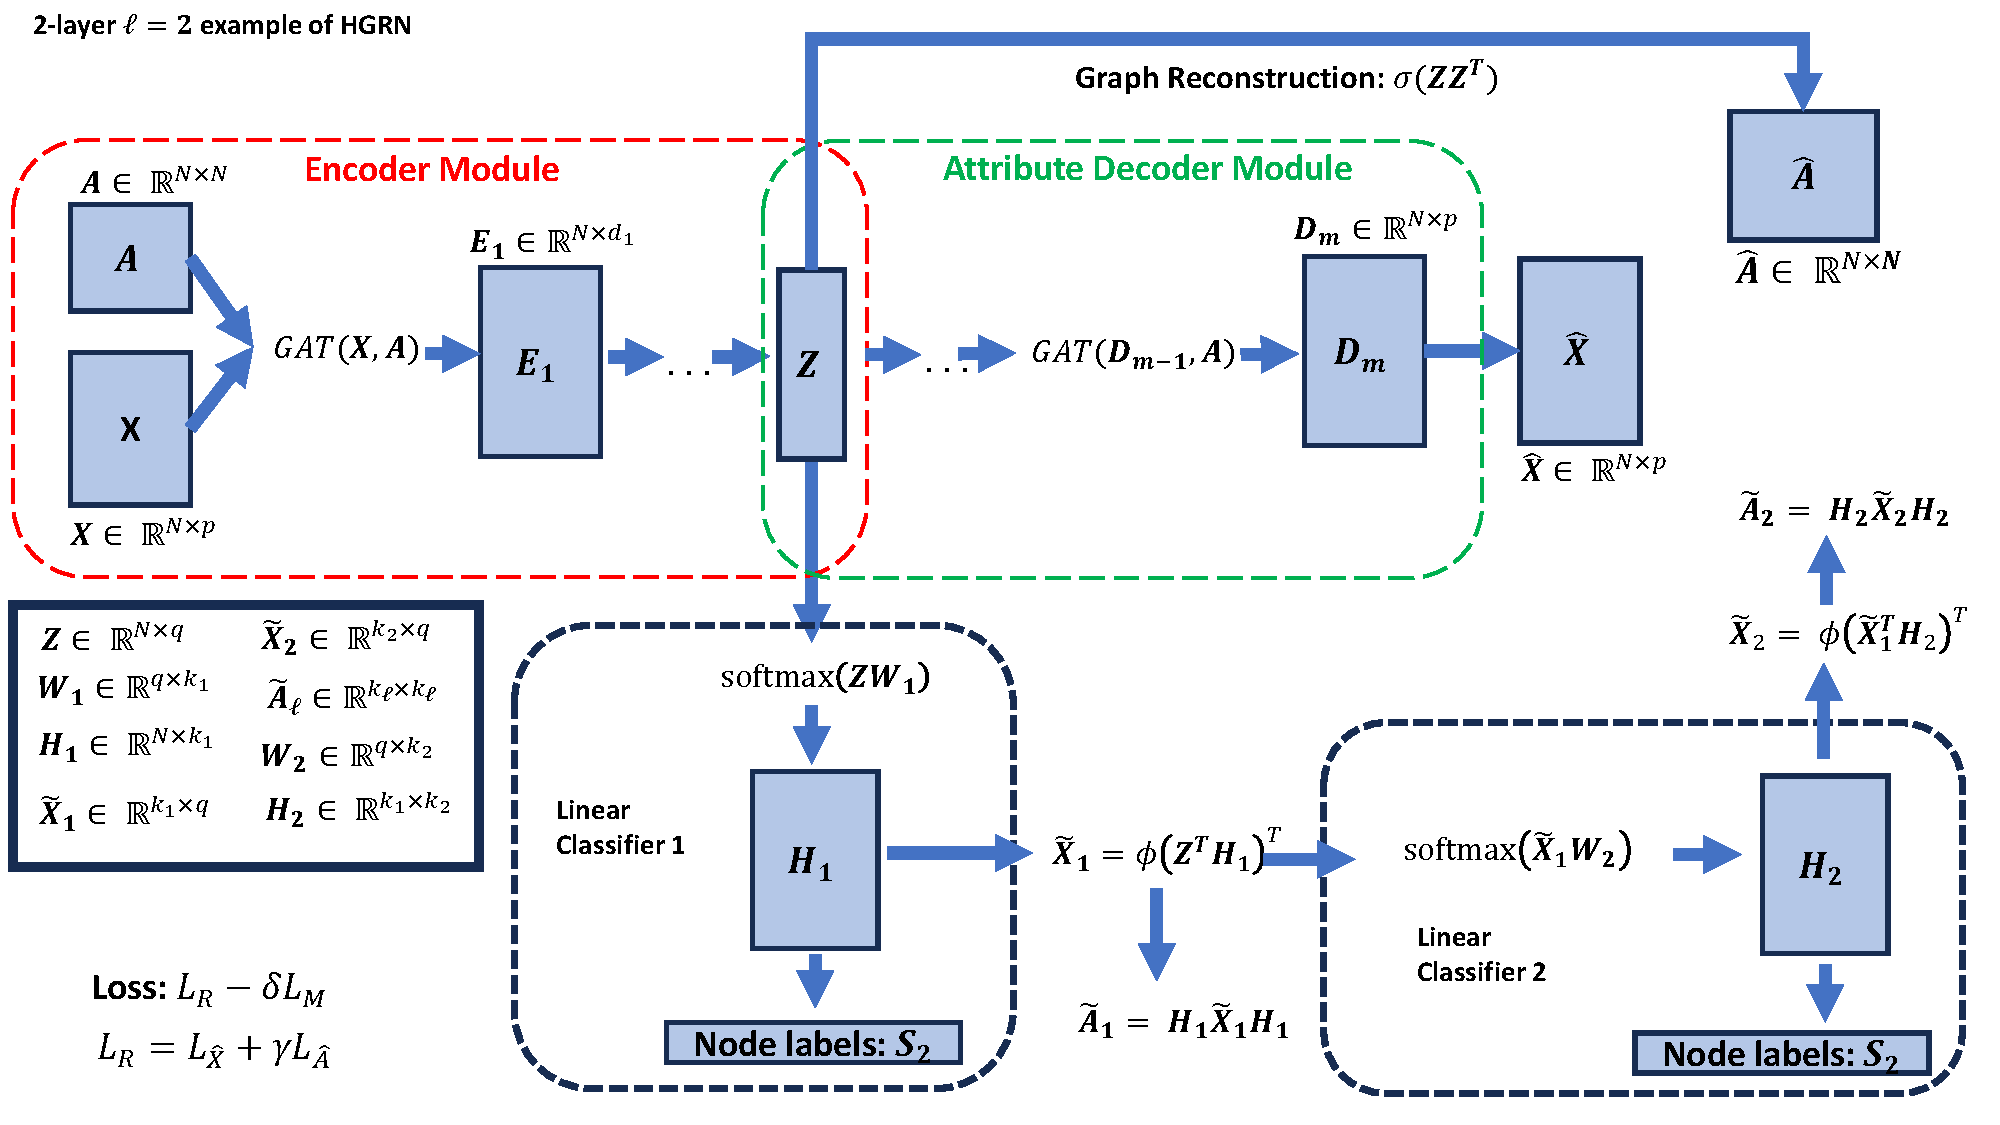
\includegraphics[scale = 0.5]{C:/Users/Bruin/Documents/GitHub/HGRN_repo/HGRN_pseudocode/HGRN_schematic2.pdf}
\end{figure}
	
	
	
	
	
	
	
	
	
	
	
	
	
	
	
	
	
	
	
	
	
	
	
	
	
	
	
	
	
	
	
	
	
	
	
	\clearpage
	\newpage
	
	\bibliographystyle{unsrt}
	\bibliography{pseudocode_bibs}
	
	
	
	
	
	
\end{document}